% LunaZen: User Guide. What the app does, how to use it, how it works in one page, why its numbers can be trusted, and what it does not do.
% This guide and the README are the project's documentation.
%
% Build (XeLaTeX, for the Inter and TeX Gyre Pagella fonts), in this folder, twice:
%   xelatex lunazen_guide.tex
%   xelatex lunazen_guide.tex
% Inter lives in \interdir (see lunazen_preamble.tex); override with: xelatex "\def\interdir{/path/to/inter/}% LunaZen: User Guide. What the app does, how to use it, how it works in one page, why its numbers can be trusted, and what it does not do.
% This guide and the README are the project's documentation.
%
% Build (XeLaTeX, for the Inter and TeX Gyre Pagella fonts), in this folder, twice:
%   xelatex lunazen_guide.tex
%   xelatex lunazen_guide.tex
% Inter lives in \interdir (see lunazen_preamble.tex); override with: xelatex "\def\interdir{/path/to/inter/}% LunaZen: User Guide. What the app does, how to use it, how it works in one page, why its numbers can be trusted, and what it does not do.
% This guide and the README are the project's documentation.
%
% Build (XeLaTeX, for the Inter and TeX Gyre Pagella fonts), in this folder, twice:
%   xelatex lunazen_guide.tex
%   xelatex lunazen_guide.tex
% Inter lives in \interdir (see lunazen_preamble.tex); override with: xelatex "\def\interdir{/path/to/inter/}% LunaZen: User Guide. What the app does, how to use it, how it works in one page, why its numbers can be trusted, and what it does not do.
% This guide and the README are the project's documentation.
%
% Build (XeLaTeX, for the Inter and TeX Gyre Pagella fonts), in this folder, twice:
%   xelatex lunazen_guide.tex
%   xelatex lunazen_guide.tex
% Inter lives in \interdir (see lunazen_preamble.tex); override with: xelatex "\def\interdir{/path/to/inter/}\input{lunazen_guide}"
% Data figures (run in this folder): node compute.mjs && uv run python figures.py   (computed with web/engine from web/data)
% App screenshots (from the repository root): uv run python docs/learn/shots.py
\newcommand{\doctitle}{LunaZen: User Guide}
\newcommand{\docsubject}{How to use the LunaZen Landing Site Navigator, and why its numbers can be trusted}
\input{lunazen_preamble}
\newcommand{\shotpair}[3]{\begin{figure}[ht]\centering
\includegraphics[width=0.485\textwidth,height=0.4\textheight,keepaspectratio]{#1}\hfill\includegraphics[width=0.485\textwidth,height=0.4\textheight,keepaspectratio]{#2}
\caption{#3}\end{figure}}
\newcommand{\shot}[2]{\begin{figure}[ht]\centering\includegraphics[width=0.485\textwidth,height=0.4\textheight,keepaspectratio]{#1}\caption{#2}\end{figure}}

\begin{document}
% ================================================================= FRONT PAGE
\thispagestyle{plain}
\pdfbookmark[0]{Overview}{overview}
\vspace*{-0.6cm}
{\sffamily\footnotesize\color{sun}\MakeUppercase{LunaZen Landing Site Navigator \quad NASA Space Apps Challenge 2026}}\par\vspace{5pt}
{\headfont\fontsize{27}{31}\selectfont LunaZen:\\[1pt] User Guide}\par\vspace{7pt}
{\large\itshape\color{muted}Where and when a lander at the lunar south pole has sunlight and a line to Earth, and how long the dark lasts}\par
\vspace{10pt}

\begin{figure}[h]
\centering\includegraphics[width=\textwidth]{hero_skyline.pdf}
\caption{Forty-five days at Site01-1 on the Connecting Ridge, from 1 March 2027, as the app computes them. The Sun circles the horizon but never climbs more than about two degrees; Earth bobs up and down in one direction. Pale points are hidden behind the terrain.}\label{fig:hero}
\end{figure}
\vspace{-4pt}

\begin{tcbraster}[raster columns=2,raster equal height=rows,raster column skip=8pt,raster row skip=8pt]
\begin{tile}{sun}{The problem}
Near the lunar south pole the Sun stays within a few degrees of the horizon and Earth skims it too. Ridges far away decide whether a lander has light and a radio link. A spot can be lit for most of the year and still face a night of days.
\end{tile}
\begin{tile}{earth}{What the app does}
For any listed spot, or your own point near the pole, on any date from 2024 to 2043, every 15 minutes: is the Sun up, is Earth up with a Deep Space Network (DSN) antenna in view, and how long does the dark last? It then answers planning questions: where to land, when, and what still works if the date slips.
\end{tile}
\begin{tile}{vermil}{What you can do with it}
Test a landing at the target and at 12 points up to 100~m around it. Compare the longest night with a limit that real missions have used. Re-plan when the date slips. Look at the real skyline in a panorama or in 3D. It all runs in your browser.
\end{tile}
\begin{tile}{ok}{Why you can rely on it}
Sun and Earth directions agree with JPL Horizons to $0.1''$. Long-term sunlight agrees with NASA's LOLA maps to $1.6$ points RMS. The Sun's angle at the Apollo moonwalks agrees to $0.12^\circ$. Every check is listed in the app's Evidence page.
\end{tile}
\end{tcbraster}

\vspace{2pt}
{\sffamily\footnotesize\color{muted}\textbf{How to read this.} Section~1: the polar sky. Sections~2 and 3: the app and three walkthroughs. Sections~4 to 6: how it works, why to trust it, what it does not do. The outline in the side panel jumps to any section.}

% ================================================================= THE POLAR SKY
\section{A Sun That Never Rises}\label{sec:problem}
On most of the Moon the Sun rises, crosses the sky and sets once a month. Near the south pole it does neither. The Moon's axis is tilted only $1.5^\circ$ from upright relative to the Sun, so from the pole the Sun circles the horizon once a month, a degree or two up at most, and passes behind each ridge in turn. Earth stays in roughly one place in the lunar sky, but the Moon's slight wobble carries it up and down by a few degrees, so Earth skims the horizon as well.

\begin{figure}[h]
\centering\includegraphics[width=\textwidth]{two_skies.pdf}
\caption{The same 30 days from 1 March 2027 at two landing sites, on the same scale. Elevations are above a flat horizon; the terrain is not shown.}\label{fig:twoskies}
\end{figure}

The pole is where many planned missions are going, because its permanently shadowed craters hold water ice and some nearby ridges are lit for most of the year. That is also why choosing a spot there is hard.

\lead{Averages hide the answer that matters.} At Site01-1 the Sun is up $89.7\%$ of 2027, yet its longest night lasts $138$~h, almost six days. That is $28$ times the $5$~h that Blue Ghost~1 survived and nearly three times the $50$~h design figure of NASA's VIPER rover. A lander has to get through its longest night, not its average day.

\lead{Small differences matter.} With the Sun so low, a tenth of a degree of horizon height can move a sunset by hours. The terrain has to be traced finely and far, the height of the antenna matters, and the Sun and Earth have to be treated as disks.

% ================================================================= USING THE APP
\section{What the App Answers}\label{sec:app}
LunaZen asks three things for a place and a stretch of time:

\begin{enumerate}[label={\sffamily\bfseries\color{sun}\arabic*.},leftmargin=1.6em]
\item \textbf{Is the Sun up?} Any part of its disk above the terrain counts, because a solar array still collects light from a partly hidden Sun.
\item \textbf{Can the lander talk to Earth?} Earth must be up, and a DSN complex (Goldstone, Madrid or Canberra) must see the Moon more than $10^\circ$ above its horizon.
\item \textbf{How long is the longest night?} It is compared with a darkness limit: $5$~h, which Blue Ghost~1 survived after sunset, $50$~h, VIPER's design figure, or any number of hours you enter.
\end{enumerate}

The pages are grouped as \textbf{Learn} (look at the sky) and \textbf{Plan} (decide). They pass your settings to each other, and every view is a link you can share.

\begin{lztable}
\begin{tabularx}{\textwidth}{@{}>{\bfseries}P{2.4cm}L@{}}
\toprule
\multicolumn{2}{@{}l}{\textbf{\color{sun}Learn}} \\
\midrule
Map & NASA's average sunlight and Earth visibility over the pole, with 13 candidate sites and 67 spots. Click a spot for a short verdict and four figures. \emph{Plot a point} adds your own location inside a mapped site; \emph{My points} keeps up to five. \\
Explorer & One spot over 1 to 365 days: the real skyline with the Sun and Earth on it, a 3D terrain view, countdowns to the next sunset and Earthset, and a timeline of Sun, Earth and DSN with exportable windows. \\
Whole Moon & Twelve landing sites away from the pole (Apollo, Chang'e, Chandrayaan-3, SLIM), each sky shown beside the pole's. \\
\midrule
\multicolumn{2}{@{}l}{\textbf{\color{earth}Plan}} \\
\midrule
Planner & When to land at one spot, asked as a sentence. Every 6-hourly landing time is tested at the spot and its dispersion points, with a verdict and the single changes that would make a window valid. \\
Rank & All 67 spots for one landing time, best first. \\
Delay impact & Whether a spot is valid on a day, how long it stays valid, when the next window opens and which other spots work. \\
Compare landings & Up to four pinned landings side by side; shift them all by some days and re-test. \\
Compare sites & Two to four sites over the same dates in one table, with Sun and DSN timelines. \\
\midrule
Resources & This guide, the checks, the data sources, scope and videos. \\
\bottomrule
\end{tabularx}
\end{lztable}

Besides the 67 spots, the app covers three flown CLPS landers (IM-1, Blue Ghost~1, IM-2) and the twelve sites away from the pole. Yearly summaries for 2027 to 2029 are precomputed and any other date from 2024 to 2043 is computed when you ask.

% ================================================================= WALKTHROUGHS
\section{Three Questions, Three Walkthroughs}\label{sec:walkthroughs}
The Plan pages open on Site01-1 from 15 March 2027 (a 14-day mission, nights under 50~h, DSN in view at least 50\%, a 2~m mast, a 100~m dispersion radius). The addresses under the figures reproduce them.

\subsection{Is this a good place to land?}
Open the \textbf{Map}, choose a site and click Site01-1. The band under the map answers in a sentence first: very bright, but with long nights. Its four figures are the sunlit share, Earth in view, the longest night (5~d 18~h) and the longest gap without a DSN station in view. To try your own location, open \emph{Plot a point}, pick a point on the map and save it to My points; it then appears on every other page.

The \textbf{Explorer} shows the same spot as a sky. At 06:15 UTC on 1 March 2027 the Sun sets in 36~h 15~min and Earth rises in 3~d 18~h. The 3D terrain tab flies over the ground lit by the Sun at that moment, and the Visibility Timeline shows how far the Sun clears the skyline, often by less than a degree.

\shotpair{app_map.png}{app_explorer.png}{Left: the Map with Site01-1 selected (\code{map.html\#spot=Site01-1}). Right: the Explorer at Site01-1, 45 days from 1 March 2027 (\code{explorer.html\#spot=Site01-1\&mast=2\&start=2027-03-01\&days=45\&t=25}).}

Where the lander touches down matters as much as where it is aimed: within 100~m of Site01-1 the yearly sunlight ranges from $33\%$ to $91\%$. The height of the antenna matters as much: at Site01-1 the longest night is $207$~h on a 1~m mast, $138$~h on 2~m and $75$~h on 10~m.

\subsection{When should we land?}
The \textbf{Planner} writes the question as a sentence whose orange words you can change: \emph{identify the earliest valid window at Site01-1 from 15 March 2027 to 14 May 2027 for a 14~d mission, max night 50~h, min DSN $\ge 50\%$, mast 2~m, 100~m dispersion radius}. Every 6-hourly landing time becomes one cell of the grid: dark green if the spot and its 12 dispersion points all pass, light green if only the spot passes, orange if the night exceeds the limit, hatched if DSN visibility is too low.

Here $18\%$ of landing times are valid at the spot, but none is valid within 100~m. The banner says why: the best landing, 9 April at 00:00 UTC, passes at the spot and at 8 of the 12 dispersion points. Under \emph{Constraint relaxation} the Planner then offers the single changes that would work, each checked by the engine: land at DM2-4 (9 valid landing days, from 7 April), accept a lander that tolerates 253~h of darkness, or tighten the dispersion radius to 50~m (2 valid landing times, from 9 April). One click applies a change; the pin icon keeps a landing for comparison.

\subsection{The launch slipped. What now?}
\textbf{Delay impact} answers the first question a slip raises. For Site01-1 on 15 March 2027 the answer is no, because DSN visibility is below the threshold. The next valid window opens on 2 April, 18 days later; the previous one was on 13 March. The table lists the other spots that are valid that day, with how long each stays valid.

\shotpair{app_planner.png}{app_windows.png}{Left: the Planner for Site01-1 from 15 March 2027 (\code{planner.html\#spot=Site01-1\&start=2027-03-15\&days=61}). Right: Delay impact for the same spot on 15 March 2027 (\code{windows.html\#spot=Site01-1\&date=2027-03-15}).}

\textbf{Compare landings} handles the slip for every option at once. Pin up to four landings in the Planner, shift them all by a number of days and each is re-tested with its own question. A nine-day slip breaks both pinned landings below: at DM2-4 the longest night grows from 37~h to 7~d 14~h, and at Site01-1 from 36~h to 3~d 15~h. Each card offers to re-pin at the next valid landing, and the exports record every question with the data version.

\shot{app_compare.png}{Compare landings after shifting two pinned landings by nine days.}

% ================================================================= HOW IT WORKS, TRUST, LIMITS
\section{How It Works in One Page}\label{sec:method}
For one moment at one place the app works in five steps, then repeats them through time.

\begin{enumerate}[label={\sffamily\bfseries\color{sun}\arabic*.},leftmargin=1.6em]
\item \textbf{Time.} The date and UTC time become ephemeris time, a uniform clock.
\item \textbf{Positions.} NASA/JPL's DE440 ephemeris, read with SPICE, gives the Sun and Earth as seen from the Moon.
\item \textbf{Directions.} Those positions become a compass direction and a height above the local horizontal at the spot.
\item \textbf{The skyline.} The terrain horizon in every direction is traced once, offline, from NASA's 5~m to 474~m elevation maps out to 300~km, for an antenna on a 2~m mast by default. The Sun and Earth are disks, so the app measures how much of each disk clears the skyline.
\item \textbf{Answers.} The Sun is up when any part of its disk is above the skyline, and Earth likewise. DSN visibility needs Earth up and a DSN complex seeing the Moon above $10^\circ$. The longest night is the longest stretch with no part of the Sun above the skyline.
\end{enumerate}

The heavy work is done once, offline: the skylines are precomputed, and the ephemeris for 2024 to 2043 is a $1.6$~MB table. The browser repeats only the cheap steps, in parallel, every 15 minutes, so a question is answered in about a second and nothing is sent to a server. A Python version is the reference and the browser's results are tested against it.

\section{Why Trust It}\label{sec:validation}
Each check compares the program with evidence it did not produce, and its tolerance is fixed in the code. The Evidence page in the app shows every check against its tolerance.

\begin{lztable}
\begin{tabularx}{\textwidth}{@{}P{3.2cm}L>{\raggedright\arraybackslash}p{4.6cm}@{}}
\toprule
\textbf{Check} & \textbf{Compared with} & \textbf{Result} \\
\midrule
Sun and Earth directions & JPL Horizons; 4 sites, 70 dates each & within $0.1''$ \\
Long-term sunlight & NASA's LOLA average-visibility maps; 26 points & $1.6$ points RMS ($2.0$ at worst on the six flattest) \\
Seven regions & Barker et al.\ (2021), peer reviewed & within $1.4$ points \\
All 67 spots & NASA's map at the same pixel & correlation $0.96$ \\
Apollo moonwalks & Apollo Lunar Surface Journal; 10 times at Apollo 11, 12, 14 & Sun angle within $0.12^\circ$ \\
Recent landings & IM-1's measured height; Blue Ghost~1's sunset & $15$~m; $6$~minutes \\
Browser and Python & the same questions asked of both & identical within a microsecond and $0.1''$ \\
\bottomrule
\end{tabularx}
\end{lztable}

\section{What It Does Not Do}\label{sec:limits}
LunaZen answers geometry questions, and it is clear about where geometry stops.
\begin{itemize}
\item \textbf{It is not a power model.} It reports light, darkness and line of sight. A lander's batteries, heaters and panels need the lander's own data, so a lander is judged only against a darkness limit with a source, or hours you enter.
\item \textbf{DSN visibility is line of sight.} Link budgets and antenna scheduling are not modelled. When Earth crosses in front of the Sun (eclipses), the Sun is dimmed for a few hours; this is not modelled either.
\item \textbf{Percentages are firmer than times.} Near the pole a small horizon error can move a sunrise by hours, so the app reports percentages and durations. The Planner, Rank and Explorer repeat the test with the skyline raised by $0.25^\circ$ to show how much a result depends on the terrain map.
\item \textbf{Terrain detail varies.} The 67 spots use NASA's 5~m maps. Sites away from the pole use a coarser 474~m map, and your own points use a 20~m copy, so their nights can differ from the 5~m result.
\end{itemize}

\section{Try It and Where to Go Next}\label{sec:reproduce}
\lead{The app} is at \appurl. To run it locally, \code{cd web \&\& npm run serve} and open \code{http://localhost:8000/}; a packaged zip runs with \code{./start.sh} or \code{start.bat}. \lead{The repository} is at \repourl, with the README, the tests and two notebooks in \code{notebooks/} that follow the method step by step. \lead{The videos}, a six-part series on the south polar sky, explain the concepts rather than the app.

\section*{References}\label{sec:refs}
\phantomsection\addcontentsline{toc}{section}{References}\markboth{References}{}
\begin{small}\sloppy
\begin{itemize}[leftmargin=1.2em,itemsep=0pt]
\item Barker, M.~K., Mazarico, E., Neumann, G.~A., Smith, D.~E., Zuber, M.~T., Head, J.~W. (2021). Improved LOLA elevation maps for south pole landing sites: error estimates and their impact on illumination conditions. \emph{Planetary and Space Science} 203, 105119. doi:10.1016/j.pss.2020.105119.
\item Mazarico, E., Neumann, G.~A., Smith, D.~E., Zuber, M.~T., Torrence, M.~H. (2011). Illumination conditions of the lunar polar regions using LOLA topography. \emph{Icarus} 211(2), 1066--1081. doi:10.1016/j.icarus.2010.10.030.
\item NASA Planetary Geodesy Data Archive. High-Resolution LOLA Topography for Lunar South Pole Sites. \url{https://pgda.gsfc.nasa.gov/products/78}.
\item LOLA average Sun and Earth visibility maps (\code{AVGVISIB\_85S\_060M\_201608}, 60~m). \url{https://imbrium.mit.edu/EXTRAS/ILLUMINATION/}.
\end{itemize}
\end{small}

\end{document}
"
% Data figures (run in this folder): node compute.mjs && uv run python figures.py   (computed with web/engine from web/data)
% App screenshots (from the repository root): uv run python docs/learn/shots.py
\newcommand{\doctitle}{LunaZen: User Guide}
\newcommand{\docsubject}{How to use the LunaZen Landing Site Navigator, and why its numbers can be trusted}
% Preamble of the User Guide (lunazen_guide.tex).
% Each document defines \doctitle and \docsubject before it inputs this file.
% Fonts: Inter and TeX Gyre Pagella (XeLaTeX). Override the Inter folder with \interdir (see the line below).
\documentclass[11pt,a4paper]{article}
\usepackage[a4paper,left=2.5cm,right=2.5cm,top=2.5cm,bottom=2.5cm,headsep=0.9cm,footskip=1.1cm]{geometry}
\usepackage{amsmath,amssymb}
\providecommand{\interdir}{/usr/share/fonts/opentype/inter/}% where Inter lives; override: xelatex "\def\interdir{/path/to/inter/}\input{how_the_app_works}"
\usepackage{mathpazo}
\usepackage[no-math]{fontspec}
\setmainfont{texgyrepagella}[Extension=.otf, UprightFont=*-regular, BoldFont=*-bold, ItalicFont=*-italic, BoldItalicFont=*-bolditalic]% TeX Live's copy, found by file name
\setsansfont{Inter}[Path=\interdir, Extension=.otf, UprightFont=*-Regular, BoldFont=*-SemiBold,
  ItalicFont=*-Italic, BoldItalicFont=*-SemiBoldItalic, Scale=MatchLowercase, RawFeature={-calt}]% no contextual alternates: Inter swaps the hyphen in "Site01-1" for a glyph that copies out as a gap
\newfontfamily\headfont{Inter}[Path=\interdir, Extension=.otf, UprightFont=*-Bold, Scale=MatchLowercase, RawFeature={-calt}]
\setmonofont{DejaVuSansMono}[Extension=.ttf, UprightFont=*, BoldFont=DejaVuSansMono-Bold, ItalicFont=DejaVuSansMono-Oblique, BoldItalicFont=DejaVuSansMono-BoldOblique, Scale=0.8]% TeX Live's copy, found by file name
\usepackage{microtype}
\setlength{\emergencystretch}{2.5em}
\usepackage{graphicx}
\usepackage[dvipsnames]{xcolor}
\usepackage{tikz}
\usetikzlibrary{arrows.meta,positioning,calc,decorations.pathreplacing}
\usepackage[most]{tcolorbox}
\usepackage{titlesec}
\usepackage{booktabs}
\usepackage{tabularx}
\usepackage{array}
\usepackage{enumitem}
\usepackage{fancyhdr}
\usepackage{needspace}
\usepackage[font={small,sf},labelfont={bf},labelsep=period,justification=raggedright,singlelinecheck=false,skip=6pt]{caption}
\graphicspath{{figures/}}

% ---------------------------------------------------------------- colour
% The app's palette: ink navy for structure, the Sun's amber and Earth's blue for meaning, vermilion only for "fails".
\definecolor{ink}{HTML}{101A33}
\definecolor{sky}{HTML}{2456C6}
\definecolor{sun}{HTML}{E69F00}
\definecolor{earth}{HTML}{0072B2}
\definecolor{vermil}{HTML}{D55E00}
\definecolor{ok}{HTML}{0B7A5A}
\definecolor{panel}{HTML}{F1F3F8}
\definecolor{rule}{HTML}{D5DAE6}
\definecolor{muted}{HTML}{5A6482}
\color{ink}

% ---------------------------------------------------------------- text
\setlength{\parindent}{0pt}
\setlength{\parskip}{5.5pt plus 1pt}
\linespread{1.08}
\setlist{nosep,leftmargin=1.4em,topsep=3pt}
\setlist[itemize]{label={\color{sun}\small$\bullet$}}
\renewcommand{\arraystretch}{1.22}
\newcommand{\vs}{\mathbf{v}}
\newcommand{\code}[1]{\texttt{#1}}
\newcommand{\lead}[1]{{\sffamily\bfseries #1}\enspace}
\newcommand{\unit}[1]{\,\mathrm{#1}}
\setcounter{secnumdepth}{2}

% ---------------------------------------------------------------- headings
\titleformat{\section}{\headfont\fontsize{15.5}{19}\selectfont\color{ink}}{\color{sun}\thesection}{0.55em}{}
\titlespacing*{\section}{0pt}{20pt}{6pt}
\titleformat{\subsection}{\sffamily\bfseries\fontsize{11.5}{14}\selectfont\color{ink}}{\color{muted}\thesubsection}{0.55em}{}
\titlespacing*{\subsection}{0pt}{12pt}{3pt}

% A part opener: a dark band, and an entry at the top level of the PDF outline.
\newcommand{\docpart}[3]{%
  \clearpage
  \phantomsection\addcontentsline{toc}{part}{#1: #2}%
  \begin{tcolorbox}[enhanced,colback=ink,colframe=ink,arc=0pt,boxrule=0pt,left=14pt,right=14pt,top=12pt,bottom=12pt,
    underlay={\fill[sun] (frame.north west) rectangle ([xshift=4pt]frame.south west);}]
  {\sffamily\footnotesize\color{sun}\MakeUppercase{#1}}\par\vspace{2pt}
  {\headfont\fontsize{20}{24}\selectfont\color{white}#2}\par\vspace{4pt}
  {\sffamily\small\color{white!82!ink}#3}
  \end{tcolorbox}\vspace{4pt}}

% ---------------------------------------------------------------- boxes
\tcbset{lzbase/.style={enhanced,breakable,arc=0pt,boxrule=0pt,left=9pt,right=9pt,top=6pt,bottom=6pt,
  fonttitle=\sffamily\bfseries\small,detach title,before upper={\tcbtitle\par\vspace{2pt}}}}
\newtcolorbox{example}[1][Worked example]{lzbase,colback=earth!6,coltitle=earth!80!black,title={#1},
  borderline west={2.5pt}{0pt}{earth}}
\newtcolorbox{aside}[1]{lzbase,colback=panel,coltitle=ink,title={#1},borderline west={2.5pt}{0pt}{sun}}
\newtcolorbox{tile}[2]{enhanced,arc=0pt,boxrule=0pt,colback=panel,left=8pt,right=8pt,top=6pt,bottom=7pt,
  borderline north={2pt}{0pt}{#1},fontupper=\small,before upper={{\sffamily\bfseries\small\color{#1!75!ink}#2}\par\vspace{2pt}},equal height group=glance}
\newcommand{\reproduce}[1]{\par\smallskip\noindent\begin{tcolorbox}[enhanced,arc=0pt,boxrule=0pt,colback=white,left=8pt,right=6pt,top=2pt,bottom=2pt,
  borderline west={2pt}{0pt}{vermil}]\sffamily\footnotesize\textbf{\color{vermil}Reproduce it (source repository).} #1\end{tcolorbox}}

% ---------------------------------------------------------------- tables
\newenvironment{lztable}{\par\smallskip\begin{center}\sffamily\footnotesize\renewcommand{\arraystretch}{1.3}}{\end{center}\smallskip}
\newcolumntype{L}{>{\raggedright\arraybackslash}X}
\newcolumntype{P}[1]{>{\raggedright\arraybackslash}p{#1}}

% ---------------------------------------------------------------- page style
\pagestyle{fancy}\fancyhf{}
\renewcommand{\headrulewidth}{0pt}
\fancyhead[L]{\sffamily\scriptsize\color{muted}\doctitle}
\fancyhead[R]{\sffamily\scriptsize\color{muted}\leftmark}
\fancyfoot[C]{\sffamily\footnotesize\color{muted}\thepage}
\renewcommand{\sectionmark}[1]{\markboth{#1}{}}
\fancypagestyle{plain}{\fancyhf{}\fancyfoot[C]{\sffamily\footnotesize\color{muted}\thepage}}

\usepackage[colorlinks=true,linkcolor=sky,urlcolor=sky,citecolor=sky,bookmarksnumbered=true,bookmarksopen=true,
  bookmarksopenlevel=1,pdfpagemode=UseOutlines,pdfdisplaydoctitle=true,
  pdftitle={\doctitle},pdfauthor={Team LunaZen},
  pdfsubject={\docsubject},
  pdfkeywords={Moon, south pole, landing sites, illumination, Earth visibility, LOLA, SPICE, NASA Space Apps}]{hyperref}
\usepackage{bookmark}
\usepackage{xurl}
% The two addresses used in the guide. Replace the placeholders (same values as web/app/site-config.js), then rebuild.
\urldef{\repourl}\url{https://github.com/lunazen-spaceapp/lunazen-v1}
\urldef{\appurl}\url{https://lunazen-v1.vercel.app}
\urlstyle{sf}


\newcommand{\shotpair}[3]{\begin{figure}[ht]\centering
\includegraphics[width=0.485\textwidth,height=0.4\textheight,keepaspectratio]{#1}\hfill\includegraphics[width=0.485\textwidth,height=0.4\textheight,keepaspectratio]{#2}
\caption{#3}\end{figure}}
\newcommand{\shot}[2]{\begin{figure}[ht]\centering\includegraphics[width=0.485\textwidth,height=0.4\textheight,keepaspectratio]{#1}\caption{#2}\end{figure}}

\begin{document}
% ================================================================= FRONT PAGE
\thispagestyle{plain}
\pdfbookmark[0]{Overview}{overview}
\vspace*{-0.6cm}
{\sffamily\footnotesize\color{sun}\MakeUppercase{LunaZen Landing Site Navigator \quad NASA Space Apps Challenge 2026}}\par\vspace{5pt}
{\headfont\fontsize{27}{31}\selectfont LunaZen:\\[1pt] User Guide}\par\vspace{7pt}
{\large\itshape\color{muted}Where and when a lander at the lunar south pole has sunlight and a line to Earth, and how long the dark lasts}\par
\vspace{10pt}

\begin{figure}[h]
\centering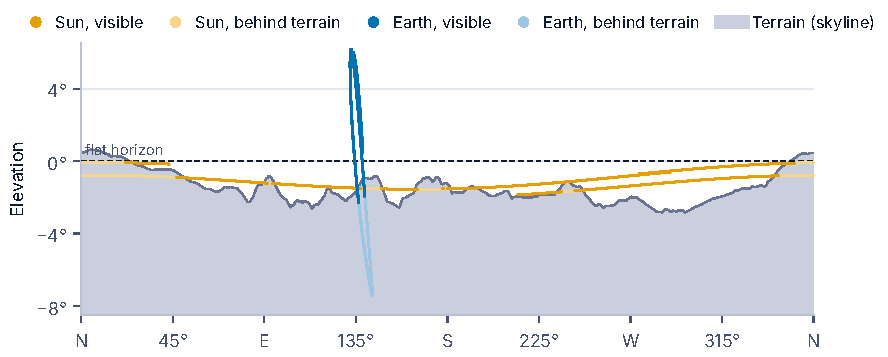
\includegraphics[width=\textwidth]{hero_skyline.pdf}
\caption{Forty-five days at Site01-1 on the Connecting Ridge, from 1 March 2027, as the app computes them. The Sun circles the horizon but never climbs more than about two degrees; Earth bobs up and down in one direction. Pale points are hidden behind the terrain.}\label{fig:hero}
\end{figure}
\vspace{-4pt}

\begin{tcbraster}[raster columns=2,raster equal height=rows,raster column skip=8pt,raster row skip=8pt]
\begin{tile}{sun}{The problem}
Near the lunar south pole the Sun stays within a few degrees of the horizon and Earth skims it too. Ridges far away decide whether a lander has light and a radio link. A spot can be lit for most of the year and still face a night of days.
\end{tile}
\begin{tile}{earth}{What the app does}
For any listed spot, or your own point near the pole, on any date from 2024 to 2043, every 15 minutes: is the Sun up, is Earth up with a Deep Space Network (DSN) antenna in view, and how long does the dark last? It then answers planning questions: where to land, when, and what still works if the date slips.
\end{tile}
\begin{tile}{vermil}{What you can do with it}
Test a landing at the target and at 12 points up to 100~m around it. Compare the longest night with a limit that real missions have used. Re-plan when the date slips. Look at the real skyline in a panorama or in 3D. It all runs in your browser.
\end{tile}
\begin{tile}{ok}{Why you can rely on it}
Sun and Earth directions agree with JPL Horizons to $0.1''$. Long-term sunlight agrees with NASA's LOLA maps to $1.6$ points RMS. The Sun's angle at the Apollo moonwalks agrees to $0.12^\circ$. Every check is listed in the app's Evidence page.
\end{tile}
\end{tcbraster}

\vspace{2pt}
{\sffamily\footnotesize\color{muted}\textbf{How to read this.} Section~1: the polar sky. Sections~2 and 3: the app and three walkthroughs. Sections~4 to 6: how it works, why to trust it, what it does not do. The outline in the side panel jumps to any section.}

% ================================================================= THE POLAR SKY
\section{A Sun That Never Rises}\label{sec:problem}
On most of the Moon the Sun rises, crosses the sky and sets once a month. Near the south pole it does neither. The Moon's axis is tilted only $1.5^\circ$ from upright relative to the Sun, so from the pole the Sun circles the horizon once a month, a degree or two up at most, and passes behind each ridge in turn. Earth stays in roughly one place in the lunar sky, but the Moon's slight wobble carries it up and down by a few degrees, so Earth skims the horizon as well.

\begin{figure}[h]
\centering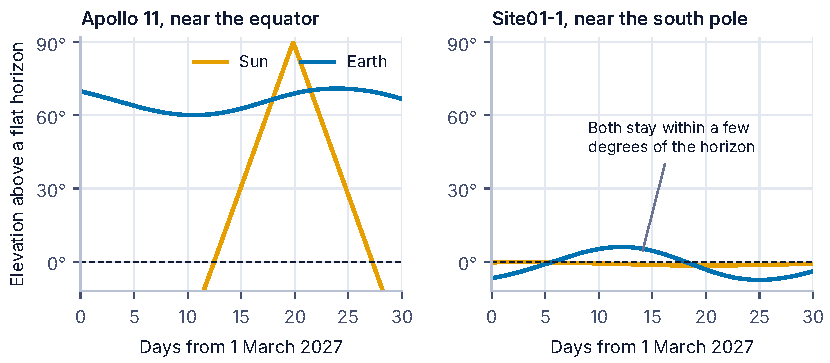
\includegraphics[width=\textwidth]{two_skies.pdf}
\caption{The same 30 days from 1 March 2027 at two landing sites, on the same scale. Elevations are above a flat horizon; the terrain is not shown.}\label{fig:twoskies}
\end{figure}

The pole is where many planned missions are going, because its permanently shadowed craters hold water ice and some nearby ridges are lit for most of the year. That is also why choosing a spot there is hard.

\lead{Averages hide the answer that matters.} At Site01-1 the Sun is up $89.7\%$ of 2027, yet its longest night lasts $138$~h, almost six days. That is $28$ times the $5$~h that Blue Ghost~1 survived and nearly three times the $50$~h design figure of NASA's VIPER rover. A lander has to get through its longest night, not its average day.

\lead{Small differences matter.} With the Sun so low, a tenth of a degree of horizon height can move a sunset by hours. The terrain has to be traced finely and far, the height of the antenna matters, and the Sun and Earth have to be treated as disks.

% ================================================================= USING THE APP
\section{What the App Answers}\label{sec:app}
LunaZen asks three things for a place and a stretch of time:

\begin{enumerate}[label={\sffamily\bfseries\color{sun}\arabic*.},leftmargin=1.6em]
\item \textbf{Is the Sun up?} Any part of its disk above the terrain counts, because a solar array still collects light from a partly hidden Sun.
\item \textbf{Can the lander talk to Earth?} Earth must be up, and a DSN complex (Goldstone, Madrid or Canberra) must see the Moon more than $10^\circ$ above its horizon.
\item \textbf{How long is the longest night?} It is compared with a darkness limit: $5$~h, which Blue Ghost~1 survived after sunset, $50$~h, VIPER's design figure, or any number of hours you enter.
\end{enumerate}

The pages are grouped as \textbf{Learn} (look at the sky) and \textbf{Plan} (decide). They pass your settings to each other, and every view is a link you can share.

\begin{lztable}
\begin{tabularx}{\textwidth}{@{}>{\bfseries}P{2.4cm}L@{}}
\toprule
\multicolumn{2}{@{}l}{\textbf{\color{sun}Learn}} \\
\midrule
Map & NASA's average sunlight and Earth visibility over the pole, with 13 candidate sites and 67 spots. Click a spot for a short verdict and four figures. \emph{Plot a point} adds your own location inside a mapped site; \emph{My points} keeps up to five. \\
Explorer & One spot over 1 to 365 days: the real skyline with the Sun and Earth on it, a 3D terrain view, countdowns to the next sunset and Earthset, and a timeline of Sun, Earth and DSN with exportable windows. \\
Whole Moon & Twelve landing sites away from the pole (Apollo, Chang'e, Chandrayaan-3, SLIM), each sky shown beside the pole's. \\
\midrule
\multicolumn{2}{@{}l}{\textbf{\color{earth}Plan}} \\
\midrule
Planner & When to land at one spot, asked as a sentence. Every 6-hourly landing time is tested at the spot and its dispersion points, with a verdict and the single changes that would make a window valid. \\
Rank & All 67 spots for one landing time, best first. \\
Delay impact & Whether a spot is valid on a day, how long it stays valid, when the next window opens and which other spots work. \\
Compare landings & Up to four pinned landings side by side; shift them all by some days and re-test. \\
Compare sites & Two to four sites over the same dates in one table, with Sun and DSN timelines. \\
\midrule
Resources & This guide, the checks, the data sources, scope and videos. \\
\bottomrule
\end{tabularx}
\end{lztable}

Besides the 67 spots, the app covers three flown CLPS landers (IM-1, Blue Ghost~1, IM-2) and the twelve sites away from the pole. Yearly summaries for 2027 to 2029 are precomputed and any other date from 2024 to 2043 is computed when you ask.

% ================================================================= WALKTHROUGHS
\section{Three Questions, Three Walkthroughs}\label{sec:walkthroughs}
The Plan pages open on Site01-1 from 15 March 2027 (a 14-day mission, nights under 50~h, DSN in view at least 50\%, a 2~m mast, a 100~m dispersion radius). The addresses under the figures reproduce them.

\subsection{Is this a good place to land?}
Open the \textbf{Map}, choose a site and click Site01-1. The band under the map answers in a sentence first: very bright, but with long nights. Its four figures are the sunlit share, Earth in view, the longest night (5~d 18~h) and the longest gap without a DSN station in view. To try your own location, open \emph{Plot a point}, pick a point on the map and save it to My points; it then appears on every other page.

The \textbf{Explorer} shows the same spot as a sky. At 06:15 UTC on 1 March 2027 the Sun sets in 36~h 15~min and Earth rises in 3~d 18~h. The 3D terrain tab flies over the ground lit by the Sun at that moment, and the Visibility Timeline shows how far the Sun clears the skyline, often by less than a degree.

\shotpair{app_map.png}{app_explorer.png}{Left: the Map with Site01-1 selected (\code{map.html\#spot=Site01-1}). Right: the Explorer at Site01-1, 45 days from 1 March 2027 (\code{explorer.html\#spot=Site01-1\&mast=2\&start=2027-03-01\&days=45\&t=25}).}

Where the lander touches down matters as much as where it is aimed: within 100~m of Site01-1 the yearly sunlight ranges from $33\%$ to $91\%$. The height of the antenna matters as much: at Site01-1 the longest night is $207$~h on a 1~m mast, $138$~h on 2~m and $75$~h on 10~m.

\subsection{When should we land?}
The \textbf{Planner} writes the question as a sentence whose orange words you can change: \emph{identify the earliest valid window at Site01-1 from 15 March 2027 to 14 May 2027 for a 14~d mission, max night 50~h, min DSN $\ge 50\%$, mast 2~m, 100~m dispersion radius}. Every 6-hourly landing time becomes one cell of the grid: dark green if the spot and its 12 dispersion points all pass, light green if only the spot passes, orange if the night exceeds the limit, hatched if DSN visibility is too low.

Here $18\%$ of landing times are valid at the spot, but none is valid within 100~m. The banner says why: the best landing, 9 April at 00:00 UTC, passes at the spot and at 8 of the 12 dispersion points. Under \emph{Constraint relaxation} the Planner then offers the single changes that would work, each checked by the engine: land at DM2-4 (9 valid landing days, from 7 April), accept a lander that tolerates 253~h of darkness, or tighten the dispersion radius to 50~m (2 valid landing times, from 9 April). One click applies a change; the pin icon keeps a landing for comparison.

\subsection{The launch slipped. What now?}
\textbf{Delay impact} answers the first question a slip raises. For Site01-1 on 15 March 2027 the answer is no, because DSN visibility is below the threshold. The next valid window opens on 2 April, 18 days later; the previous one was on 13 March. The table lists the other spots that are valid that day, with how long each stays valid.

\shotpair{app_planner.png}{app_windows.png}{Left: the Planner for Site01-1 from 15 March 2027 (\code{planner.html\#spot=Site01-1\&start=2027-03-15\&days=61}). Right: Delay impact for the same spot on 15 March 2027 (\code{windows.html\#spot=Site01-1\&date=2027-03-15}).}

\textbf{Compare landings} handles the slip for every option at once. Pin up to four landings in the Planner, shift them all by a number of days and each is re-tested with its own question. A nine-day slip breaks both pinned landings below: at DM2-4 the longest night grows from 37~h to 7~d 14~h, and at Site01-1 from 36~h to 3~d 15~h. Each card offers to re-pin at the next valid landing, and the exports record every question with the data version.

\shot{app_compare.png}{Compare landings after shifting two pinned landings by nine days.}

% ================================================================= HOW IT WORKS, TRUST, LIMITS
\section{How It Works in One Page}\label{sec:method}
For one moment at one place the app works in five steps, then repeats them through time.

\begin{enumerate}[label={\sffamily\bfseries\color{sun}\arabic*.},leftmargin=1.6em]
\item \textbf{Time.} The date and UTC time become ephemeris time, a uniform clock.
\item \textbf{Positions.} NASA/JPL's DE440 ephemeris, read with SPICE, gives the Sun and Earth as seen from the Moon.
\item \textbf{Directions.} Those positions become a compass direction and a height above the local horizontal at the spot.
\item \textbf{The skyline.} The terrain horizon in every direction is traced once, offline, from NASA's 5~m to 474~m elevation maps out to 300~km, for an antenna on a 2~m mast by default. The Sun and Earth are disks, so the app measures how much of each disk clears the skyline.
\item \textbf{Answers.} The Sun is up when any part of its disk is above the skyline, and Earth likewise. DSN visibility needs Earth up and a DSN complex seeing the Moon above $10^\circ$. The longest night is the longest stretch with no part of the Sun above the skyline.
\end{enumerate}

The heavy work is done once, offline: the skylines are precomputed, and the ephemeris for 2024 to 2043 is a $1.6$~MB table. The browser repeats only the cheap steps, in parallel, every 15 minutes, so a question is answered in about a second and nothing is sent to a server. A Python version is the reference and the browser's results are tested against it.

\section{Why Trust It}\label{sec:validation}
Each check compares the program with evidence it did not produce, and its tolerance is fixed in the code. The Evidence page in the app shows every check against its tolerance.

\begin{lztable}
\begin{tabularx}{\textwidth}{@{}P{3.2cm}L>{\raggedright\arraybackslash}p{4.6cm}@{}}
\toprule
\textbf{Check} & \textbf{Compared with} & \textbf{Result} \\
\midrule
Sun and Earth directions & JPL Horizons; 4 sites, 70 dates each & within $0.1''$ \\
Long-term sunlight & NASA's LOLA average-visibility maps; 26 points & $1.6$ points RMS ($2.0$ at worst on the six flattest) \\
Seven regions & Barker et al.\ (2021), peer reviewed & within $1.4$ points \\
All 67 spots & NASA's map at the same pixel & correlation $0.96$ \\
Apollo moonwalks & Apollo Lunar Surface Journal; 10 times at Apollo 11, 12, 14 & Sun angle within $0.12^\circ$ \\
Recent landings & IM-1's measured height; Blue Ghost~1's sunset & $15$~m; $6$~minutes \\
Browser and Python & the same questions asked of both & identical within a microsecond and $0.1''$ \\
\bottomrule
\end{tabularx}
\end{lztable}

\section{What It Does Not Do}\label{sec:limits}
LunaZen answers geometry questions, and it is clear about where geometry stops.
\begin{itemize}
\item \textbf{It is not a power model.} It reports light, darkness and line of sight. A lander's batteries, heaters and panels need the lander's own data, so a lander is judged only against a darkness limit with a source, or hours you enter.
\item \textbf{DSN visibility is line of sight.} Link budgets and antenna scheduling are not modelled. When Earth crosses in front of the Sun (eclipses), the Sun is dimmed for a few hours; this is not modelled either.
\item \textbf{Percentages are firmer than times.} Near the pole a small horizon error can move a sunrise by hours, so the app reports percentages and durations. The Planner, Rank and Explorer repeat the test with the skyline raised by $0.25^\circ$ to show how much a result depends on the terrain map.
\item \textbf{Terrain detail varies.} The 67 spots use NASA's 5~m maps. Sites away from the pole use a coarser 474~m map, and your own points use a 20~m copy, so their nights can differ from the 5~m result.
\end{itemize}

\section{Try It and Where to Go Next}\label{sec:reproduce}
\lead{The app} is at \appurl. To run it locally, \code{cd web \&\& npm run serve} and open \code{http://localhost:8000/}; a packaged zip runs with \code{./start.sh} or \code{start.bat}. \lead{The repository} is at \repourl, with the README, the tests and two notebooks in \code{notebooks/} that follow the method step by step. \lead{The videos}, a six-part series on the south polar sky, explain the concepts rather than the app.

\section*{References}\label{sec:refs}
\phantomsection\addcontentsline{toc}{section}{References}\markboth{References}{}
\begin{small}\sloppy
\begin{itemize}[leftmargin=1.2em,itemsep=0pt]
\item Barker, M.~K., Mazarico, E., Neumann, G.~A., Smith, D.~E., Zuber, M.~T., Head, J.~W. (2021). Improved LOLA elevation maps for south pole landing sites: error estimates and their impact on illumination conditions. \emph{Planetary and Space Science} 203, 105119. doi:10.1016/j.pss.2020.105119.
\item Mazarico, E., Neumann, G.~A., Smith, D.~E., Zuber, M.~T., Torrence, M.~H. (2011). Illumination conditions of the lunar polar regions using LOLA topography. \emph{Icarus} 211(2), 1066--1081. doi:10.1016/j.icarus.2010.10.030.
\item NASA Planetary Geodesy Data Archive. High-Resolution LOLA Topography for Lunar South Pole Sites. \url{https://pgda.gsfc.nasa.gov/products/78}.
\item LOLA average Sun and Earth visibility maps (\code{AVGVISIB\_85S\_060M\_201608}, 60~m). \url{https://imbrium.mit.edu/EXTRAS/ILLUMINATION/}.
\end{itemize}
\end{small}

\end{document}
"
% Data figures (run in this folder): node compute.mjs && uv run python figures.py   (computed with web/engine from web/data)
% App screenshots (from the repository root): uv run python docs/learn/shots.py
\newcommand{\doctitle}{LunaZen: User Guide}
\newcommand{\docsubject}{How to use the LunaZen Landing Site Navigator, and why its numbers can be trusted}
% Preamble of the User Guide (lunazen_guide.tex).
% Each document defines \doctitle and \docsubject before it inputs this file.
% Fonts: Inter and TeX Gyre Pagella (XeLaTeX). Override the Inter folder with \interdir (see the line below).
\documentclass[11pt,a4paper]{article}
\usepackage[a4paper,left=2.5cm,right=2.5cm,top=2.5cm,bottom=2.5cm,headsep=0.9cm,footskip=1.1cm]{geometry}
\usepackage{amsmath,amssymb}
\providecommand{\interdir}{/usr/share/fonts/opentype/inter/}% where Inter lives; override: xelatex "\def\interdir{/path/to/inter/}\input{how_the_app_works}"
\usepackage{mathpazo}
\usepackage[no-math]{fontspec}
\setmainfont{texgyrepagella}[Extension=.otf, UprightFont=*-regular, BoldFont=*-bold, ItalicFont=*-italic, BoldItalicFont=*-bolditalic]% TeX Live's copy, found by file name
\setsansfont{Inter}[Path=\interdir, Extension=.otf, UprightFont=*-Regular, BoldFont=*-SemiBold,
  ItalicFont=*-Italic, BoldItalicFont=*-SemiBoldItalic, Scale=MatchLowercase, RawFeature={-calt}]% no contextual alternates: Inter swaps the hyphen in "Site01-1" for a glyph that copies out as a gap
\newfontfamily\headfont{Inter}[Path=\interdir, Extension=.otf, UprightFont=*-Bold, Scale=MatchLowercase, RawFeature={-calt}]
\setmonofont{DejaVuSansMono}[Extension=.ttf, UprightFont=*, BoldFont=DejaVuSansMono-Bold, ItalicFont=DejaVuSansMono-Oblique, BoldItalicFont=DejaVuSansMono-BoldOblique, Scale=0.8]% TeX Live's copy, found by file name
\usepackage{microtype}
\setlength{\emergencystretch}{2.5em}
\usepackage{graphicx}
\usepackage[dvipsnames]{xcolor}
\usepackage{tikz}
\usetikzlibrary{arrows.meta,positioning,calc,decorations.pathreplacing}
\usepackage[most]{tcolorbox}
\usepackage{titlesec}
\usepackage{booktabs}
\usepackage{tabularx}
\usepackage{array}
\usepackage{enumitem}
\usepackage{fancyhdr}
\usepackage{needspace}
\usepackage[font={small,sf},labelfont={bf},labelsep=period,justification=raggedright,singlelinecheck=false,skip=6pt]{caption}
\graphicspath{{figures/}}

% ---------------------------------------------------------------- colour
% The app's palette: ink navy for structure, the Sun's amber and Earth's blue for meaning, vermilion only for "fails".
\definecolor{ink}{HTML}{101A33}
\definecolor{sky}{HTML}{2456C6}
\definecolor{sun}{HTML}{E69F00}
\definecolor{earth}{HTML}{0072B2}
\definecolor{vermil}{HTML}{D55E00}
\definecolor{ok}{HTML}{0B7A5A}
\definecolor{panel}{HTML}{F1F3F8}
\definecolor{rule}{HTML}{D5DAE6}
\definecolor{muted}{HTML}{5A6482}
\color{ink}

% ---------------------------------------------------------------- text
\setlength{\parindent}{0pt}
\setlength{\parskip}{5.5pt plus 1pt}
\linespread{1.08}
\setlist{nosep,leftmargin=1.4em,topsep=3pt}
\setlist[itemize]{label={\color{sun}\small$\bullet$}}
\renewcommand{\arraystretch}{1.22}
\newcommand{\vs}{\mathbf{v}}
\newcommand{\code}[1]{\texttt{#1}}
\newcommand{\lead}[1]{{\sffamily\bfseries #1}\enspace}
\newcommand{\unit}[1]{\,\mathrm{#1}}
\setcounter{secnumdepth}{2}

% ---------------------------------------------------------------- headings
\titleformat{\section}{\headfont\fontsize{15.5}{19}\selectfont\color{ink}}{\color{sun}\thesection}{0.55em}{}
\titlespacing*{\section}{0pt}{20pt}{6pt}
\titleformat{\subsection}{\sffamily\bfseries\fontsize{11.5}{14}\selectfont\color{ink}}{\color{muted}\thesubsection}{0.55em}{}
\titlespacing*{\subsection}{0pt}{12pt}{3pt}

% A part opener: a dark band, and an entry at the top level of the PDF outline.
\newcommand{\docpart}[3]{%
  \clearpage
  \phantomsection\addcontentsline{toc}{part}{#1: #2}%
  \begin{tcolorbox}[enhanced,colback=ink,colframe=ink,arc=0pt,boxrule=0pt,left=14pt,right=14pt,top=12pt,bottom=12pt,
    underlay={\fill[sun] (frame.north west) rectangle ([xshift=4pt]frame.south west);}]
  {\sffamily\footnotesize\color{sun}\MakeUppercase{#1}}\par\vspace{2pt}
  {\headfont\fontsize{20}{24}\selectfont\color{white}#2}\par\vspace{4pt}
  {\sffamily\small\color{white!82!ink}#3}
  \end{tcolorbox}\vspace{4pt}}

% ---------------------------------------------------------------- boxes
\tcbset{lzbase/.style={enhanced,breakable,arc=0pt,boxrule=0pt,left=9pt,right=9pt,top=6pt,bottom=6pt,
  fonttitle=\sffamily\bfseries\small,detach title,before upper={\tcbtitle\par\vspace{2pt}}}}
\newtcolorbox{example}[1][Worked example]{lzbase,colback=earth!6,coltitle=earth!80!black,title={#1},
  borderline west={2.5pt}{0pt}{earth}}
\newtcolorbox{aside}[1]{lzbase,colback=panel,coltitle=ink,title={#1},borderline west={2.5pt}{0pt}{sun}}
\newtcolorbox{tile}[2]{enhanced,arc=0pt,boxrule=0pt,colback=panel,left=8pt,right=8pt,top=6pt,bottom=7pt,
  borderline north={2pt}{0pt}{#1},fontupper=\small,before upper={{\sffamily\bfseries\small\color{#1!75!ink}#2}\par\vspace{2pt}},equal height group=glance}
\newcommand{\reproduce}[1]{\par\smallskip\noindent\begin{tcolorbox}[enhanced,arc=0pt,boxrule=0pt,colback=white,left=8pt,right=6pt,top=2pt,bottom=2pt,
  borderline west={2pt}{0pt}{vermil}]\sffamily\footnotesize\textbf{\color{vermil}Reproduce it (source repository).} #1\end{tcolorbox}}

% ---------------------------------------------------------------- tables
\newenvironment{lztable}{\par\smallskip\begin{center}\sffamily\footnotesize\renewcommand{\arraystretch}{1.3}}{\end{center}\smallskip}
\newcolumntype{L}{>{\raggedright\arraybackslash}X}
\newcolumntype{P}[1]{>{\raggedright\arraybackslash}p{#1}}

% ---------------------------------------------------------------- page style
\pagestyle{fancy}\fancyhf{}
\renewcommand{\headrulewidth}{0pt}
\fancyhead[L]{\sffamily\scriptsize\color{muted}\doctitle}
\fancyhead[R]{\sffamily\scriptsize\color{muted}\leftmark}
\fancyfoot[C]{\sffamily\footnotesize\color{muted}\thepage}
\renewcommand{\sectionmark}[1]{\markboth{#1}{}}
\fancypagestyle{plain}{\fancyhf{}\fancyfoot[C]{\sffamily\footnotesize\color{muted}\thepage}}

\usepackage[colorlinks=true,linkcolor=sky,urlcolor=sky,citecolor=sky,bookmarksnumbered=true,bookmarksopen=true,
  bookmarksopenlevel=1,pdfpagemode=UseOutlines,pdfdisplaydoctitle=true,
  pdftitle={\doctitle},pdfauthor={Team LunaZen},
  pdfsubject={\docsubject},
  pdfkeywords={Moon, south pole, landing sites, illumination, Earth visibility, LOLA, SPICE, NASA Space Apps}]{hyperref}
\usepackage{bookmark}
\usepackage{xurl}
% The two addresses used in the guide. Replace the placeholders (same values as web/app/site-config.js), then rebuild.
\urldef{\repourl}\url{https://github.com/lunazen-spaceapp/lunazen-v1}
\urldef{\appurl}\url{https://lunazen-v1.vercel.app}
\urlstyle{sf}


\newcommand{\shotpair}[3]{\begin{figure}[ht]\centering
\includegraphics[width=0.485\textwidth,height=0.4\textheight,keepaspectratio]{#1}\hfill\includegraphics[width=0.485\textwidth,height=0.4\textheight,keepaspectratio]{#2}
\caption{#3}\end{figure}}
\newcommand{\shot}[2]{\begin{figure}[ht]\centering\includegraphics[width=0.485\textwidth,height=0.4\textheight,keepaspectratio]{#1}\caption{#2}\end{figure}}

\begin{document}
% ================================================================= FRONT PAGE
\thispagestyle{plain}
\pdfbookmark[0]{Overview}{overview}
\vspace*{-0.6cm}
{\sffamily\footnotesize\color{sun}\MakeUppercase{LunaZen Landing Site Navigator \quad NASA Space Apps Challenge 2026}}\par\vspace{5pt}
{\headfont\fontsize{27}{31}\selectfont LunaZen:\\[1pt] User Guide}\par\vspace{7pt}
{\large\itshape\color{muted}Where and when a lander at the lunar south pole has sunlight and a line to Earth, and how long the dark lasts}\par
\vspace{10pt}

\begin{figure}[h]
\centering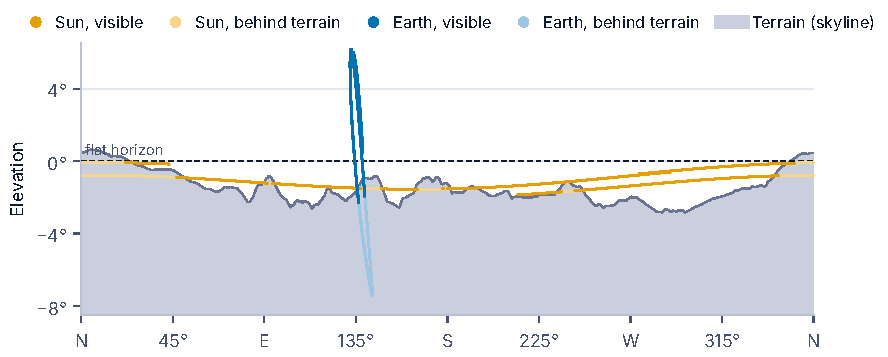
\includegraphics[width=\textwidth]{hero_skyline.pdf}
\caption{Forty-five days at Site01-1 on the Connecting Ridge, from 1 March 2027, as the app computes them. The Sun circles the horizon but never climbs more than about two degrees; Earth bobs up and down in one direction. Pale points are hidden behind the terrain.}\label{fig:hero}
\end{figure}
\vspace{-4pt}

\begin{tcbraster}[raster columns=2,raster equal height=rows,raster column skip=8pt,raster row skip=8pt]
\begin{tile}{sun}{The problem}
Near the lunar south pole the Sun stays within a few degrees of the horizon and Earth skims it too. Ridges far away decide whether a lander has light and a radio link. A spot can be lit for most of the year and still face a night of days.
\end{tile}
\begin{tile}{earth}{What the app does}
For any listed spot, or your own point near the pole, on any date from 2024 to 2043, every 15 minutes: is the Sun up, is Earth up with a Deep Space Network (DSN) antenna in view, and how long does the dark last? It then answers planning questions: where to land, when, and what still works if the date slips.
\end{tile}
\begin{tile}{vermil}{What you can do with it}
Test a landing at the target and at 12 points up to 100~m around it. Compare the longest night with a limit that real missions have used. Re-plan when the date slips. Look at the real skyline in a panorama or in 3D. It all runs in your browser.
\end{tile}
\begin{tile}{ok}{Why you can rely on it}
Sun and Earth directions agree with JPL Horizons to $0.1''$. Long-term sunlight agrees with NASA's LOLA maps to $1.6$ points RMS. The Sun's angle at the Apollo moonwalks agrees to $0.12^\circ$. Every check is listed in the app's Evidence page.
\end{tile}
\end{tcbraster}

\vspace{2pt}
{\sffamily\footnotesize\color{muted}\textbf{How to read this.} Section~1: the polar sky. Sections~2 and 3: the app and three walkthroughs. Sections~4 to 6: how it works, why to trust it, what it does not do. The outline in the side panel jumps to any section.}

% ================================================================= THE POLAR SKY
\section{A Sun That Never Rises}\label{sec:problem}
On most of the Moon the Sun rises, crosses the sky and sets once a month. Near the south pole it does neither. The Moon's axis is tilted only $1.5^\circ$ from upright relative to the Sun, so from the pole the Sun circles the horizon once a month, a degree or two up at most, and passes behind each ridge in turn. Earth stays in roughly one place in the lunar sky, but the Moon's slight wobble carries it up and down by a few degrees, so Earth skims the horizon as well.

\begin{figure}[h]
\centering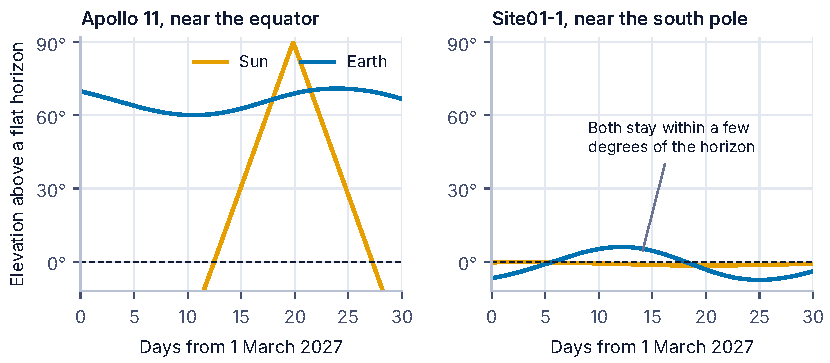
\includegraphics[width=\textwidth]{two_skies.pdf}
\caption{The same 30 days from 1 March 2027 at two landing sites, on the same scale. Elevations are above a flat horizon; the terrain is not shown.}\label{fig:twoskies}
\end{figure}

The pole is where many planned missions are going, because its permanently shadowed craters hold water ice and some nearby ridges are lit for most of the year. That is also why choosing a spot there is hard.

\lead{Averages hide the answer that matters.} At Site01-1 the Sun is up $89.7\%$ of 2027, yet its longest night lasts $138$~h, almost six days. That is $28$ times the $5$~h that Blue Ghost~1 survived and nearly three times the $50$~h design figure of NASA's VIPER rover. A lander has to get through its longest night, not its average day.

\lead{Small differences matter.} With the Sun so low, a tenth of a degree of horizon height can move a sunset by hours. The terrain has to be traced finely and far, the height of the antenna matters, and the Sun and Earth have to be treated as disks.

% ================================================================= USING THE APP
\section{What the App Answers}\label{sec:app}
LunaZen asks three things for a place and a stretch of time:

\begin{enumerate}[label={\sffamily\bfseries\color{sun}\arabic*.},leftmargin=1.6em]
\item \textbf{Is the Sun up?} Any part of its disk above the terrain counts, because a solar array still collects light from a partly hidden Sun.
\item \textbf{Can the lander talk to Earth?} Earth must be up, and a DSN complex (Goldstone, Madrid or Canberra) must see the Moon more than $10^\circ$ above its horizon.
\item \textbf{How long is the longest night?} It is compared with a darkness limit: $5$~h, which Blue Ghost~1 survived after sunset, $50$~h, VIPER's design figure, or any number of hours you enter.
\end{enumerate}

The pages are grouped as \textbf{Learn} (look at the sky) and \textbf{Plan} (decide). They pass your settings to each other, and every view is a link you can share.

\begin{lztable}
\begin{tabularx}{\textwidth}{@{}>{\bfseries}P{2.4cm}L@{}}
\toprule
\multicolumn{2}{@{}l}{\textbf{\color{sun}Learn}} \\
\midrule
Map & NASA's average sunlight and Earth visibility over the pole, with 13 candidate sites and 67 spots. Click a spot for a short verdict and four figures. \emph{Plot a point} adds your own location inside a mapped site; \emph{My points} keeps up to five. \\
Explorer & One spot over 1 to 365 days: the real skyline with the Sun and Earth on it, a 3D terrain view, countdowns to the next sunset and Earthset, and a timeline of Sun, Earth and DSN with exportable windows. \\
Whole Moon & Twelve landing sites away from the pole (Apollo, Chang'e, Chandrayaan-3, SLIM), each sky shown beside the pole's. \\
\midrule
\multicolumn{2}{@{}l}{\textbf{\color{earth}Plan}} \\
\midrule
Planner & When to land at one spot, asked as a sentence. Every 6-hourly landing time is tested at the spot and its dispersion points, with a verdict and the single changes that would make a window valid. \\
Rank & All 67 spots for one landing time, best first. \\
Delay impact & Whether a spot is valid on a day, how long it stays valid, when the next window opens and which other spots work. \\
Compare landings & Up to four pinned landings side by side; shift them all by some days and re-test. \\
Compare sites & Two to four sites over the same dates in one table, with Sun and DSN timelines. \\
\midrule
Resources & This guide, the checks, the data sources, scope and videos. \\
\bottomrule
\end{tabularx}
\end{lztable}

Besides the 67 spots, the app covers three flown CLPS landers (IM-1, Blue Ghost~1, IM-2) and the twelve sites away from the pole. Yearly summaries for 2027 to 2029 are precomputed and any other date from 2024 to 2043 is computed when you ask.

% ================================================================= WALKTHROUGHS
\section{Three Questions, Three Walkthroughs}\label{sec:walkthroughs}
The Plan pages open on Site01-1 from 15 March 2027 (a 14-day mission, nights under 50~h, DSN in view at least 50\%, a 2~m mast, a 100~m dispersion radius). The addresses under the figures reproduce them.

\subsection{Is this a good place to land?}
Open the \textbf{Map}, choose a site and click Site01-1. The band under the map answers in a sentence first: very bright, but with long nights. Its four figures are the sunlit share, Earth in view, the longest night (5~d 18~h) and the longest gap without a DSN station in view. To try your own location, open \emph{Plot a point}, pick a point on the map and save it to My points; it then appears on every other page.

The \textbf{Explorer} shows the same spot as a sky. At 06:15 UTC on 1 March 2027 the Sun sets in 36~h 15~min and Earth rises in 3~d 18~h. The 3D terrain tab flies over the ground lit by the Sun at that moment, and the Visibility Timeline shows how far the Sun clears the skyline, often by less than a degree.

\shotpair{app_map.png}{app_explorer.png}{Left: the Map with Site01-1 selected (\code{map.html\#spot=Site01-1}). Right: the Explorer at Site01-1, 45 days from 1 March 2027 (\code{explorer.html\#spot=Site01-1\&mast=2\&start=2027-03-01\&days=45\&t=25}).}

Where the lander touches down matters as much as where it is aimed: within 100~m of Site01-1 the yearly sunlight ranges from $33\%$ to $91\%$. The height of the antenna matters as much: at Site01-1 the longest night is $207$~h on a 1~m mast, $138$~h on 2~m and $75$~h on 10~m.

\subsection{When should we land?}
The \textbf{Planner} writes the question as a sentence whose orange words you can change: \emph{identify the earliest valid window at Site01-1 from 15 March 2027 to 14 May 2027 for a 14~d mission, max night 50~h, min DSN $\ge 50\%$, mast 2~m, 100~m dispersion radius}. Every 6-hourly landing time becomes one cell of the grid: dark green if the spot and its 12 dispersion points all pass, light green if only the spot passes, orange if the night exceeds the limit, hatched if DSN visibility is too low.

Here $18\%$ of landing times are valid at the spot, but none is valid within 100~m. The banner says why: the best landing, 9 April at 00:00 UTC, passes at the spot and at 8 of the 12 dispersion points. Under \emph{Constraint relaxation} the Planner then offers the single changes that would work, each checked by the engine: land at DM2-4 (9 valid landing days, from 7 April), accept a lander that tolerates 253~h of darkness, or tighten the dispersion radius to 50~m (2 valid landing times, from 9 April). One click applies a change; the pin icon keeps a landing for comparison.

\subsection{The launch slipped. What now?}
\textbf{Delay impact} answers the first question a slip raises. For Site01-1 on 15 March 2027 the answer is no, because DSN visibility is below the threshold. The next valid window opens on 2 April, 18 days later; the previous one was on 13 March. The table lists the other spots that are valid that day, with how long each stays valid.

\shotpair{app_planner.png}{app_windows.png}{Left: the Planner for Site01-1 from 15 March 2027 (\code{planner.html\#spot=Site01-1\&start=2027-03-15\&days=61}). Right: Delay impact for the same spot on 15 March 2027 (\code{windows.html\#spot=Site01-1\&date=2027-03-15}).}

\textbf{Compare landings} handles the slip for every option at once. Pin up to four landings in the Planner, shift them all by a number of days and each is re-tested with its own question. A nine-day slip breaks both pinned landings below: at DM2-4 the longest night grows from 37~h to 7~d 14~h, and at Site01-1 from 36~h to 3~d 15~h. Each card offers to re-pin at the next valid landing, and the exports record every question with the data version.

\shot{app_compare.png}{Compare landings after shifting two pinned landings by nine days.}

% ================================================================= HOW IT WORKS, TRUST, LIMITS
\section{How It Works in One Page}\label{sec:method}
For one moment at one place the app works in five steps, then repeats them through time.

\begin{enumerate}[label={\sffamily\bfseries\color{sun}\arabic*.},leftmargin=1.6em]
\item \textbf{Time.} The date and UTC time become ephemeris time, a uniform clock.
\item \textbf{Positions.} NASA/JPL's DE440 ephemeris, read with SPICE, gives the Sun and Earth as seen from the Moon.
\item \textbf{Directions.} Those positions become a compass direction and a height above the local horizontal at the spot.
\item \textbf{The skyline.} The terrain horizon in every direction is traced once, offline, from NASA's 5~m to 474~m elevation maps out to 300~km, for an antenna on a 2~m mast by default. The Sun and Earth are disks, so the app measures how much of each disk clears the skyline.
\item \textbf{Answers.} The Sun is up when any part of its disk is above the skyline, and Earth likewise. DSN visibility needs Earth up and a DSN complex seeing the Moon above $10^\circ$. The longest night is the longest stretch with no part of the Sun above the skyline.
\end{enumerate}

The heavy work is done once, offline: the skylines are precomputed, and the ephemeris for 2024 to 2043 is a $1.6$~MB table. The browser repeats only the cheap steps, in parallel, every 15 minutes, so a question is answered in about a second and nothing is sent to a server. A Python version is the reference and the browser's results are tested against it.

\section{Why Trust It}\label{sec:validation}
Each check compares the program with evidence it did not produce, and its tolerance is fixed in the code. The Evidence page in the app shows every check against its tolerance.

\begin{lztable}
\begin{tabularx}{\textwidth}{@{}P{3.2cm}L>{\raggedright\arraybackslash}p{4.6cm}@{}}
\toprule
\textbf{Check} & \textbf{Compared with} & \textbf{Result} \\
\midrule
Sun and Earth directions & JPL Horizons; 4 sites, 70 dates each & within $0.1''$ \\
Long-term sunlight & NASA's LOLA average-visibility maps; 26 points & $1.6$ points RMS ($2.0$ at worst on the six flattest) \\
Seven regions & Barker et al.\ (2021), peer reviewed & within $1.4$ points \\
All 67 spots & NASA's map at the same pixel & correlation $0.96$ \\
Apollo moonwalks & Apollo Lunar Surface Journal; 10 times at Apollo 11, 12, 14 & Sun angle within $0.12^\circ$ \\
Recent landings & IM-1's measured height; Blue Ghost~1's sunset & $15$~m; $6$~minutes \\
Browser and Python & the same questions asked of both & identical within a microsecond and $0.1''$ \\
\bottomrule
\end{tabularx}
\end{lztable}

\section{What It Does Not Do}\label{sec:limits}
LunaZen answers geometry questions, and it is clear about where geometry stops.
\begin{itemize}
\item \textbf{It is not a power model.} It reports light, darkness and line of sight. A lander's batteries, heaters and panels need the lander's own data, so a lander is judged only against a darkness limit with a source, or hours you enter.
\item \textbf{DSN visibility is line of sight.} Link budgets and antenna scheduling are not modelled. When Earth crosses in front of the Sun (eclipses), the Sun is dimmed for a few hours; this is not modelled either.
\item \textbf{Percentages are firmer than times.} Near the pole a small horizon error can move a sunrise by hours, so the app reports percentages and durations. The Planner, Rank and Explorer repeat the test with the skyline raised by $0.25^\circ$ to show how much a result depends on the terrain map.
\item \textbf{Terrain detail varies.} The 67 spots use NASA's 5~m maps. Sites away from the pole use a coarser 474~m map, and your own points use a 20~m copy, so their nights can differ from the 5~m result.
\end{itemize}

\section{Try It and Where to Go Next}\label{sec:reproduce}
\lead{The app} is at \appurl. To run it locally, \code{cd web \&\& npm run serve} and open \code{http://localhost:8000/}; a packaged zip runs with \code{./start.sh} or \code{start.bat}. \lead{The repository} is at \repourl, with the README, the tests and two notebooks in \code{notebooks/} that follow the method step by step. \lead{The videos}, a six-part series on the south polar sky, explain the concepts rather than the app.

\section*{References}\label{sec:refs}
\phantomsection\addcontentsline{toc}{section}{References}\markboth{References}{}
\begin{small}\sloppy
\begin{itemize}[leftmargin=1.2em,itemsep=0pt]
\item Barker, M.~K., Mazarico, E., Neumann, G.~A., Smith, D.~E., Zuber, M.~T., Head, J.~W. (2021). Improved LOLA elevation maps for south pole landing sites: error estimates and their impact on illumination conditions. \emph{Planetary and Space Science} 203, 105119. doi:10.1016/j.pss.2020.105119.
\item Mazarico, E., Neumann, G.~A., Smith, D.~E., Zuber, M.~T., Torrence, M.~H. (2011). Illumination conditions of the lunar polar regions using LOLA topography. \emph{Icarus} 211(2), 1066--1081. doi:10.1016/j.icarus.2010.10.030.
\item NASA Planetary Geodesy Data Archive. High-Resolution LOLA Topography for Lunar South Pole Sites. \url{https://pgda.gsfc.nasa.gov/products/78}.
\item LOLA average Sun and Earth visibility maps (\code{AVGVISIB\_85S\_060M\_201608}, 60~m). \url{https://imbrium.mit.edu/EXTRAS/ILLUMINATION/}.
\end{itemize}
\end{small}

\end{document}
"
% Data figures (run in this folder): node compute.mjs && uv run python figures.py   (computed with web/engine from web/data)
% App screenshots (from the repository root): uv run python docs/learn/shots.py
\newcommand{\doctitle}{LunaZen: User Guide}
\newcommand{\docsubject}{How to use the LunaZen Landing Site Navigator, and why its numbers can be trusted}
% Preamble of the User Guide (lunazen_guide.tex).
% Each document defines \doctitle and \docsubject before it inputs this file.
% Fonts: Inter and TeX Gyre Pagella (XeLaTeX). Override the Inter folder with \interdir (see the line below).
\documentclass[11pt,a4paper]{article}
\usepackage[a4paper,left=2.5cm,right=2.5cm,top=2.5cm,bottom=2.5cm,headsep=0.9cm,footskip=1.1cm]{geometry}
\usepackage{amsmath,amssymb}
\providecommand{\interdir}{/usr/share/fonts/opentype/inter/}% where Inter lives; override: xelatex "\def\interdir{/path/to/inter/}\input{how_the_app_works}"
\usepackage{mathpazo}
\usepackage[no-math]{fontspec}
\setmainfont{texgyrepagella}[Extension=.otf, UprightFont=*-regular, BoldFont=*-bold, ItalicFont=*-italic, BoldItalicFont=*-bolditalic]% TeX Live's copy, found by file name
\setsansfont{Inter}[Path=\interdir, Extension=.otf, UprightFont=*-Regular, BoldFont=*-SemiBold,
  ItalicFont=*-Italic, BoldItalicFont=*-SemiBoldItalic, Scale=MatchLowercase, RawFeature={-calt}]% no contextual alternates: Inter swaps the hyphen in "Site01-1" for a glyph that copies out as a gap
\newfontfamily\headfont{Inter}[Path=\interdir, Extension=.otf, UprightFont=*-Bold, Scale=MatchLowercase, RawFeature={-calt}]
\setmonofont{DejaVuSansMono}[Extension=.ttf, UprightFont=*, BoldFont=DejaVuSansMono-Bold, ItalicFont=DejaVuSansMono-Oblique, BoldItalicFont=DejaVuSansMono-BoldOblique, Scale=0.8]% TeX Live's copy, found by file name
\usepackage{microtype}
\setlength{\emergencystretch}{2.5em}
\usepackage{graphicx}
\usepackage[dvipsnames]{xcolor}
\usepackage{tikz}
\usetikzlibrary{arrows.meta,positioning,calc,decorations.pathreplacing}
\usepackage[most]{tcolorbox}
\usepackage{titlesec}
\usepackage{booktabs}
\usepackage{tabularx}
\usepackage{array}
\usepackage{enumitem}
\usepackage{fancyhdr}
\usepackage{needspace}
\usepackage[font={small,sf},labelfont={bf},labelsep=period,justification=raggedright,singlelinecheck=false,skip=6pt]{caption}
\graphicspath{{figures/}}

% ---------------------------------------------------------------- colour
% The app's palette: ink navy for structure, the Sun's amber and Earth's blue for meaning, vermilion only for "fails".
\definecolor{ink}{HTML}{101A33}
\definecolor{sky}{HTML}{2456C6}
\definecolor{sun}{HTML}{E69F00}
\definecolor{earth}{HTML}{0072B2}
\definecolor{vermil}{HTML}{D55E00}
\definecolor{ok}{HTML}{0B7A5A}
\definecolor{panel}{HTML}{F1F3F8}
\definecolor{rule}{HTML}{D5DAE6}
\definecolor{muted}{HTML}{5A6482}
\color{ink}

% ---------------------------------------------------------------- text
\setlength{\parindent}{0pt}
\setlength{\parskip}{5.5pt plus 1pt}
\linespread{1.08}
\setlist{nosep,leftmargin=1.4em,topsep=3pt}
\setlist[itemize]{label={\color{sun}\small$\bullet$}}
\renewcommand{\arraystretch}{1.22}
\newcommand{\vs}{\mathbf{v}}
\newcommand{\code}[1]{\texttt{#1}}
\newcommand{\lead}[1]{{\sffamily\bfseries #1}\enspace}
\newcommand{\unit}[1]{\,\mathrm{#1}}
\setcounter{secnumdepth}{2}

% ---------------------------------------------------------------- headings
\titleformat{\section}{\headfont\fontsize{15.5}{19}\selectfont\color{ink}}{\color{sun}\thesection}{0.55em}{}
\titlespacing*{\section}{0pt}{20pt}{6pt}
\titleformat{\subsection}{\sffamily\bfseries\fontsize{11.5}{14}\selectfont\color{ink}}{\color{muted}\thesubsection}{0.55em}{}
\titlespacing*{\subsection}{0pt}{12pt}{3pt}

% A part opener: a dark band, and an entry at the top level of the PDF outline.
\newcommand{\docpart}[3]{%
  \clearpage
  \phantomsection\addcontentsline{toc}{part}{#1: #2}%
  \begin{tcolorbox}[enhanced,colback=ink,colframe=ink,arc=0pt,boxrule=0pt,left=14pt,right=14pt,top=12pt,bottom=12pt,
    underlay={\fill[sun] (frame.north west) rectangle ([xshift=4pt]frame.south west);}]
  {\sffamily\footnotesize\color{sun}\MakeUppercase{#1}}\par\vspace{2pt}
  {\headfont\fontsize{20}{24}\selectfont\color{white}#2}\par\vspace{4pt}
  {\sffamily\small\color{white!82!ink}#3}
  \end{tcolorbox}\vspace{4pt}}

% ---------------------------------------------------------------- boxes
\tcbset{lzbase/.style={enhanced,breakable,arc=0pt,boxrule=0pt,left=9pt,right=9pt,top=6pt,bottom=6pt,
  fonttitle=\sffamily\bfseries\small,detach title,before upper={\tcbtitle\par\vspace{2pt}}}}
\newtcolorbox{example}[1][Worked example]{lzbase,colback=earth!6,coltitle=earth!80!black,title={#1},
  borderline west={2.5pt}{0pt}{earth}}
\newtcolorbox{aside}[1]{lzbase,colback=panel,coltitle=ink,title={#1},borderline west={2.5pt}{0pt}{sun}}
\newtcolorbox{tile}[2]{enhanced,arc=0pt,boxrule=0pt,colback=panel,left=8pt,right=8pt,top=6pt,bottom=7pt,
  borderline north={2pt}{0pt}{#1},fontupper=\small,before upper={{\sffamily\bfseries\small\color{#1!75!ink}#2}\par\vspace{2pt}},equal height group=glance}
\newcommand{\reproduce}[1]{\par\smallskip\noindent\begin{tcolorbox}[enhanced,arc=0pt,boxrule=0pt,colback=white,left=8pt,right=6pt,top=2pt,bottom=2pt,
  borderline west={2pt}{0pt}{vermil}]\sffamily\footnotesize\textbf{\color{vermil}Reproduce it (source repository).} #1\end{tcolorbox}}

% ---------------------------------------------------------------- tables
\newenvironment{lztable}{\par\smallskip\begin{center}\sffamily\footnotesize\renewcommand{\arraystretch}{1.3}}{\end{center}\smallskip}
\newcolumntype{L}{>{\raggedright\arraybackslash}X}
\newcolumntype{P}[1]{>{\raggedright\arraybackslash}p{#1}}

% ---------------------------------------------------------------- page style
\pagestyle{fancy}\fancyhf{}
\renewcommand{\headrulewidth}{0pt}
\fancyhead[L]{\sffamily\scriptsize\color{muted}\doctitle}
\fancyhead[R]{\sffamily\scriptsize\color{muted}\leftmark}
\fancyfoot[C]{\sffamily\footnotesize\color{muted}\thepage}
\renewcommand{\sectionmark}[1]{\markboth{#1}{}}
\fancypagestyle{plain}{\fancyhf{}\fancyfoot[C]{\sffamily\footnotesize\color{muted}\thepage}}

\usepackage[colorlinks=true,linkcolor=sky,urlcolor=sky,citecolor=sky,bookmarksnumbered=true,bookmarksopen=true,
  bookmarksopenlevel=1,pdfpagemode=UseOutlines,pdfdisplaydoctitle=true,
  pdftitle={\doctitle},pdfauthor={Team LunaZen},
  pdfsubject={\docsubject},
  pdfkeywords={Moon, south pole, landing sites, illumination, Earth visibility, LOLA, SPICE, NASA Space Apps}]{hyperref}
\usepackage{bookmark}
\usepackage{xurl}
% The two addresses used in the guide. Replace the placeholders (same values as web/app/site-config.js), then rebuild.
\urldef{\repourl}\url{https://github.com/lunazen-spaceapp/lunazen-v1}
\urldef{\appurl}\url{https://lunazen-v1.vercel.app}
\urlstyle{sf}


\newcommand{\shotpair}[3]{\begin{figure}[ht]\centering
\includegraphics[width=0.485\textwidth,height=0.4\textheight,keepaspectratio]{#1}\hfill\includegraphics[width=0.485\textwidth,height=0.4\textheight,keepaspectratio]{#2}
\caption{#3}\end{figure}}
\newcommand{\shot}[2]{\begin{figure}[ht]\centering\includegraphics[width=0.485\textwidth,height=0.4\textheight,keepaspectratio]{#1}\caption{#2}\end{figure}}

\begin{document}
% ================================================================= FRONT PAGE
\thispagestyle{plain}
\pdfbookmark[0]{Overview}{overview}
\vspace*{-0.6cm}
{\sffamily\footnotesize\color{sun}\MakeUppercase{LunaZen Landing Site Navigator \quad NASA Space Apps Challenge 2026}}\par\vspace{5pt}
{\headfont\fontsize{27}{31}\selectfont LunaZen:\\[1pt] User Guide}\par\vspace{7pt}
{\large\itshape\color{muted}Where and when a lander at the lunar south pole has sunlight and a line to Earth, and how long the dark lasts}\par
\vspace{10pt}

\begin{figure}[h]
\centering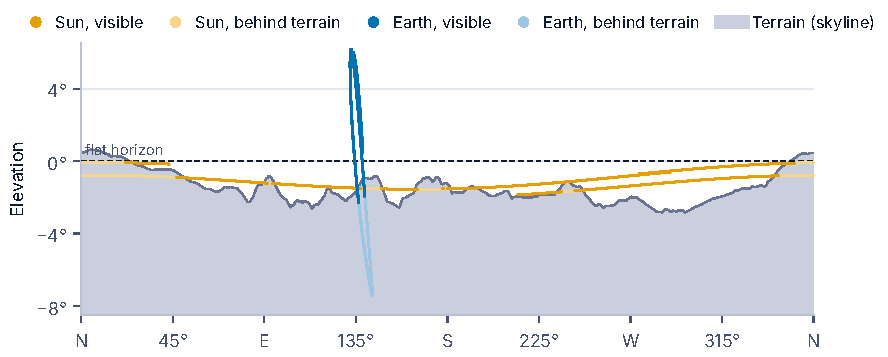
\includegraphics[width=\textwidth]{hero_skyline.pdf}
\caption{Forty-five days at Site01-1 on the Connecting Ridge, from 1 March 2027, as the app computes them. The Sun circles the horizon but never climbs more than about two degrees; Earth bobs up and down in one direction. Pale points are hidden behind the terrain.}\label{fig:hero}
\end{figure}
\vspace{-4pt}

\begin{tcbraster}[raster columns=2,raster equal height=rows,raster column skip=8pt,raster row skip=8pt]
\begin{tile}{sun}{The problem}
Near the lunar south pole the Sun stays within a few degrees of the horizon and Earth skims it too. Ridges far away decide whether a lander has light and a radio link. A spot can be lit for most of the year and still face a night of days.
\end{tile}
\begin{tile}{earth}{What the app does}
For any listed spot, or your own point near the pole, on any date from 2024 to 2043, every 15 minutes: is the Sun up, is Earth up with a Deep Space Network (DSN) antenna in view, and how long does the dark last? It then answers planning questions: where to land, when, and what still works if the date slips.
\end{tile}
\begin{tile}{vermil}{What you can do with it}
Test a landing at the target and at 12 points up to 100~m around it. Compare the longest night with a limit that real missions have used. Re-plan when the date slips. Look at the real skyline in a panorama or in 3D. It all runs in your browser.
\end{tile}
\begin{tile}{ok}{Why you can rely on it}
Sun and Earth directions agree with JPL Horizons to $0.1''$. Long-term sunlight agrees with NASA's LOLA maps to $1.6$ points RMS. The Sun's angle at the Apollo moonwalks agrees to $0.12^\circ$. Every check is listed in the app's Evidence page.
\end{tile}
\end{tcbraster}

\vspace{2pt}
{\sffamily\footnotesize\color{muted}\textbf{How to read this.} Section~1: the polar sky. Sections~2 and 3: the app and three walkthroughs. Sections~4 to 6: how it works, why to trust it, what it does not do. The outline in the side panel jumps to any section.}

% ================================================================= THE POLAR SKY
\section{A Sun That Never Rises}\label{sec:problem}
On most of the Moon the Sun rises, crosses the sky and sets once a month. Near the south pole it does neither. The Moon's axis is tilted only $1.5^\circ$ from upright relative to the Sun, so from the pole the Sun circles the horizon once a month, a degree or two up at most, and passes behind each ridge in turn. Earth stays in roughly one place in the lunar sky, but the Moon's slight wobble carries it up and down by a few degrees, so Earth skims the horizon as well.

\begin{figure}[h]
\centering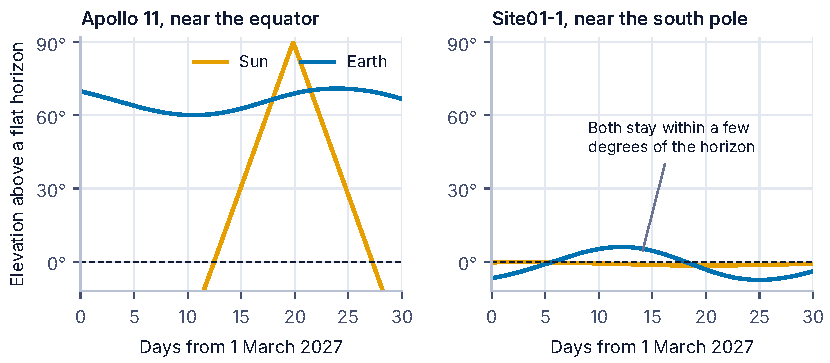
\includegraphics[width=\textwidth]{two_skies.pdf}
\caption{The same 30 days from 1 March 2027 at two landing sites, on the same scale. Elevations are above a flat horizon; the terrain is not shown.}\label{fig:twoskies}
\end{figure}

The pole is where many planned missions are going, because its permanently shadowed craters hold water ice and some nearby ridges are lit for most of the year. That is also why choosing a spot there is hard.

\lead{Averages hide the answer that matters.} At Site01-1 the Sun is up $89.7\%$ of 2027, yet its longest night lasts $138$~h, almost six days. That is $28$ times the $5$~h that Blue Ghost~1 survived and nearly three times the $50$~h design figure of NASA's VIPER rover. A lander has to get through its longest night, not its average day.

\lead{Small differences matter.} With the Sun so low, a tenth of a degree of horizon height can move a sunset by hours. The terrain has to be traced finely and far, the height of the antenna matters, and the Sun and Earth have to be treated as disks.

% ================================================================= USING THE APP
\section{What the App Answers}\label{sec:app}
LunaZen asks three things for a place and a stretch of time:

\begin{enumerate}[label={\sffamily\bfseries\color{sun}\arabic*.},leftmargin=1.6em]
\item \textbf{Is the Sun up?} Any part of its disk above the terrain counts, because a solar array still collects light from a partly hidden Sun.
\item \textbf{Can the lander talk to Earth?} Earth must be up, and a DSN complex (Goldstone, Madrid or Canberra) must see the Moon more than $10^\circ$ above its horizon.
\item \textbf{How long is the longest night?} It is compared with a darkness limit: $5$~h, which Blue Ghost~1 survived after sunset, $50$~h, VIPER's design figure, or any number of hours you enter.
\end{enumerate}

The pages are grouped as \textbf{Learn} (look at the sky) and \textbf{Plan} (decide). They pass your settings to each other, and every view is a link you can share.

\begin{lztable}
\begin{tabularx}{\textwidth}{@{}>{\bfseries}P{2.4cm}L@{}}
\toprule
\multicolumn{2}{@{}l}{\textbf{\color{sun}Learn}} \\
\midrule
Map & NASA's average sunlight and Earth visibility over the pole, with 13 candidate sites and 67 spots. Click a spot for a short verdict and four figures. \emph{Plot a point} adds your own location inside a mapped site; \emph{My points} keeps up to five. \\
Explorer & One spot over 1 to 365 days: the real skyline with the Sun and Earth on it, a 3D terrain view, countdowns to the next sunset and Earthset, and a timeline of Sun, Earth and DSN with exportable windows. \\
Whole Moon & Twelve landing sites away from the pole (Apollo, Chang'e, Chandrayaan-3, SLIM), each sky shown beside the pole's. \\
\midrule
\multicolumn{2}{@{}l}{\textbf{\color{earth}Plan}} \\
\midrule
Planner & When to land at one spot, asked as a sentence. Every 6-hourly landing time is tested at the spot and its dispersion points, with a verdict and the single changes that would make a window valid. \\
Rank & All 67 spots for one landing time, best first. \\
Delay impact & Whether a spot is valid on a day, how long it stays valid, when the next window opens and which other spots work. \\
Compare landings & Up to four pinned landings side by side; shift them all by some days and re-test. \\
Compare sites & Two to four sites over the same dates in one table, with Sun and DSN timelines. \\
\midrule
Resources & This guide, the checks, the data sources, scope and videos. \\
\bottomrule
\end{tabularx}
\end{lztable}

Besides the 67 spots, the app covers three flown CLPS landers (IM-1, Blue Ghost~1, IM-2) and the twelve sites away from the pole. Yearly summaries for 2027 to 2029 are precomputed and any other date from 2024 to 2043 is computed when you ask.

% ================================================================= WALKTHROUGHS
\section{Three Questions, Three Walkthroughs}\label{sec:walkthroughs}
The Plan pages open on Site01-1 from 15 March 2027 (a 14-day mission, nights under 50~h, DSN in view at least 50\%, a 2~m mast, a 100~m dispersion radius). The addresses under the figures reproduce them.

\subsection{Is this a good place to land?}
Open the \textbf{Map}, choose a site and click Site01-1. The band under the map answers in a sentence first: very bright, but with long nights. Its four figures are the sunlit share, Earth in view, the longest night (5~d 18~h) and the longest gap without a DSN station in view. To try your own location, open \emph{Plot a point}, pick a point on the map and save it to My points; it then appears on every other page.

The \textbf{Explorer} shows the same spot as a sky. At 06:15 UTC on 1 March 2027 the Sun sets in 36~h 15~min and Earth rises in 3~d 18~h. The 3D terrain tab flies over the ground lit by the Sun at that moment, and the Visibility Timeline shows how far the Sun clears the skyline, often by less than a degree.

\shotpair{app_map.png}{app_explorer.png}{Left: the Map with Site01-1 selected (\code{map.html\#spot=Site01-1}). Right: the Explorer at Site01-1, 45 days from 1 March 2027 (\code{explorer.html\#spot=Site01-1\&mast=2\&start=2027-03-01\&days=45\&t=25}).}

Where the lander touches down matters as much as where it is aimed: within 100~m of Site01-1 the yearly sunlight ranges from $33\%$ to $91\%$. The height of the antenna matters as much: at Site01-1 the longest night is $207$~h on a 1~m mast, $138$~h on 2~m and $75$~h on 10~m.

\subsection{When should we land?}
The \textbf{Planner} writes the question as a sentence whose orange words you can change: \emph{identify the earliest valid window at Site01-1 from 15 March 2027 to 14 May 2027 for a 14~d mission, max night 50~h, min DSN $\ge 50\%$, mast 2~m, 100~m dispersion radius}. Every 6-hourly landing time becomes one cell of the grid: dark green if the spot and its 12 dispersion points all pass, light green if only the spot passes, orange if the night exceeds the limit, hatched if DSN visibility is too low.

Here $18\%$ of landing times are valid at the spot, but none is valid within 100~m. The banner says why: the best landing, 9 April at 00:00 UTC, passes at the spot and at 8 of the 12 dispersion points. Under \emph{Constraint relaxation} the Planner then offers the single changes that would work, each checked by the engine: land at DM2-4 (9 valid landing days, from 7 April), accept a lander that tolerates 253~h of darkness, or tighten the dispersion radius to 50~m (2 valid landing times, from 9 April). One click applies a change; the pin icon keeps a landing for comparison.

\subsection{The launch slipped. What now?}
\textbf{Delay impact} answers the first question a slip raises. For Site01-1 on 15 March 2027 the answer is no, because DSN visibility is below the threshold. The next valid window opens on 2 April, 18 days later; the previous one was on 13 March. The table lists the other spots that are valid that day, with how long each stays valid.

\shotpair{app_planner.png}{app_windows.png}{Left: the Planner for Site01-1 from 15 March 2027 (\code{planner.html\#spot=Site01-1\&start=2027-03-15\&days=61}). Right: Delay impact for the same spot on 15 March 2027 (\code{windows.html\#spot=Site01-1\&date=2027-03-15}).}

\textbf{Compare landings} handles the slip for every option at once. Pin up to four landings in the Planner, shift them all by a number of days and each is re-tested with its own question. A nine-day slip breaks both pinned landings below: at DM2-4 the longest night grows from 37~h to 7~d 14~h, and at Site01-1 from 36~h to 3~d 15~h. Each card offers to re-pin at the next valid landing, and the exports record every question with the data version.

\shot{app_compare.png}{Compare landings after shifting two pinned landings by nine days.}

% ================================================================= HOW IT WORKS, TRUST, LIMITS
\section{How It Works in One Page}\label{sec:method}
For one moment at one place the app works in five steps, then repeats them through time.

\begin{enumerate}[label={\sffamily\bfseries\color{sun}\arabic*.},leftmargin=1.6em]
\item \textbf{Time.} The date and UTC time become ephemeris time, a uniform clock.
\item \textbf{Positions.} NASA/JPL's DE440 ephemeris, read with SPICE, gives the Sun and Earth as seen from the Moon.
\item \textbf{Directions.} Those positions become a compass direction and a height above the local horizontal at the spot.
\item \textbf{The skyline.} The terrain horizon in every direction is traced once, offline, from NASA's 5~m to 474~m elevation maps out to 300~km, for an antenna on a 2~m mast by default. The Sun and Earth are disks, so the app measures how much of each disk clears the skyline.
\item \textbf{Answers.} The Sun is up when any part of its disk is above the skyline, and Earth likewise. DSN visibility needs Earth up and a DSN complex seeing the Moon above $10^\circ$. The longest night is the longest stretch with no part of the Sun above the skyline.
\end{enumerate}

The heavy work is done once, offline: the skylines are precomputed, and the ephemeris for 2024 to 2043 is a $1.6$~MB table. The browser repeats only the cheap steps, in parallel, every 15 minutes, so a question is answered in about a second and nothing is sent to a server. A Python version is the reference and the browser's results are tested against it.

\section{Why Trust It}\label{sec:validation}
Each check compares the program with evidence it did not produce, and its tolerance is fixed in the code. The Evidence page in the app shows every check against its tolerance.

\begin{lztable}
\begin{tabularx}{\textwidth}{@{}P{3.2cm}L>{\raggedright\arraybackslash}p{4.6cm}@{}}
\toprule
\textbf{Check} & \textbf{Compared with} & \textbf{Result} \\
\midrule
Sun and Earth directions & JPL Horizons; 4 sites, 70 dates each & within $0.1''$ \\
Long-term sunlight & NASA's LOLA average-visibility maps; 26 points & $1.6$ points RMS ($2.0$ at worst on the six flattest) \\
Seven regions & Barker et al.\ (2021), peer reviewed & within $1.4$ points \\
All 67 spots & NASA's map at the same pixel & correlation $0.96$ \\
Apollo moonwalks & Apollo Lunar Surface Journal; 10 times at Apollo 11, 12, 14 & Sun angle within $0.12^\circ$ \\
Recent landings & IM-1's measured height; Blue Ghost~1's sunset & $15$~m; $6$~minutes \\
Browser and Python & the same questions asked of both & identical within a microsecond and $0.1''$ \\
\bottomrule
\end{tabularx}
\end{lztable}

\section{What It Does Not Do}\label{sec:limits}
LunaZen answers geometry questions, and it is clear about where geometry stops.
\begin{itemize}
\item \textbf{It is not a power model.} It reports light, darkness and line of sight. A lander's batteries, heaters and panels need the lander's own data, so a lander is judged only against a darkness limit with a source, or hours you enter.
\item \textbf{DSN visibility is line of sight.} Link budgets and antenna scheduling are not modelled. When Earth crosses in front of the Sun (eclipses), the Sun is dimmed for a few hours; this is not modelled either.
\item \textbf{Percentages are firmer than times.} Near the pole a small horizon error can move a sunrise by hours, so the app reports percentages and durations. The Planner, Rank and Explorer repeat the test with the skyline raised by $0.25^\circ$ to show how much a result depends on the terrain map.
\item \textbf{Terrain detail varies.} The 67 spots use NASA's 5~m maps. Sites away from the pole use a coarser 474~m map, and your own points use a 20~m copy, so their nights can differ from the 5~m result.
\end{itemize}

\section{Try It and Where to Go Next}\label{sec:reproduce}
\lead{The app} is at \appurl. To run it locally, \code{cd web \&\& npm run serve} and open \code{http://localhost:8000/}; a packaged zip runs with \code{./start.sh} or \code{start.bat}. \lead{The repository} is at \repourl, with the README, the tests and two notebooks in \code{notebooks/} that follow the method step by step. \lead{The videos}, a six-part series on the south polar sky, explain the concepts rather than the app.

\section*{References}\label{sec:refs}
\phantomsection\addcontentsline{toc}{section}{References}\markboth{References}{}
\begin{small}\sloppy
\begin{itemize}[leftmargin=1.2em,itemsep=0pt]
\item Barker, M.~K., Mazarico, E., Neumann, G.~A., Smith, D.~E., Zuber, M.~T., Head, J.~W. (2021). Improved LOLA elevation maps for south pole landing sites: error estimates and their impact on illumination conditions. \emph{Planetary and Space Science} 203, 105119. doi:10.1016/j.pss.2020.105119.
\item Mazarico, E., Neumann, G.~A., Smith, D.~E., Zuber, M.~T., Torrence, M.~H. (2011). Illumination conditions of the lunar polar regions using LOLA topography. \emph{Icarus} 211(2), 1066--1081. doi:10.1016/j.icarus.2010.10.030.
\item NASA Planetary Geodesy Data Archive. High-Resolution LOLA Topography for Lunar South Pole Sites. \url{https://pgda.gsfc.nasa.gov/products/78}.
\item LOLA average Sun and Earth visibility maps (\code{AVGVISIB\_85S\_060M\_201608}, 60~m). \url{https://imbrium.mit.edu/EXTRAS/ILLUMINATION/}.
\end{itemize}
\end{small}

\end{document}
